

The promise of neural solvers is to reduce time-to-solution compared with classical methods for batched PF and OPF problems. We therefore evaluate solver runtime and residuals across batches of PF and OPF instances and grid sizes, reflecting realistic utility workloads where large collections of scenarios are repeatedly solved for applications such as planning, time-series forecasting, contingency analysis, and uncertainty quantification, rather than a single isolated operating point. Since the datasets used in \cref{subsec:pf} and~\ref{subsec:opf} do not include DC solutions, we use \datakit datasets, which provide solutions obtained with all classical AC-PF/AC-OPF and DC-PF/DC-OPF solvers implemented through PowerModels~\cite{powermodels}. This enables comparison against the PowerModels implementations of AC-PF (Newton--Raphson), AC-OPF (IPOPT with MUMPS), DC-PF, and DC-OPF\footnote{A fully controlled comparison of runtime and residuals with other neural solvers from the literature remains challenging because prior work uses different benchmarking protocols and heterogeneous hardware and inputs.}. All GENCO models are trained from scratch for each task and grid.

\subsubsection{Batch Runtime Analysis Methodology}

\begin{figure*}[t]
    \centering
    % Requires in the preamble:
    % \usepackage{graphicx}
    % \usepackage{tikz}
    % \usetikzlibrary{arrows.meta,positioning,fit,calc}
    \resizebox{\textwidth}{!}{%
    \begin{tikzpicture}[
        >=Latex,
        font=\large,
        node distance=5mm and 8mm,
        every node/.style={align=center},
        box/.style={
            draw,
            rounded corners,
            minimum width=1.3cm,
            minimum height=8mm,
            inner sep=3pt,
            fill=white
        },
        sidebox/.style={
            draw,
            rounded corners,
            minimum width=3.1cm,
            minimum height=8mm,
            inner sep=3pt,
            fill=white
        },
        titlebox/.style={
            draw,
            rounded corners,
            font=\large\bfseries,
            minimum width=1.3cm,
            minimum height=9mm,
            inner sep=3pt,
            fill=white
        },
        metricbox/.style={
            draw,
            rounded corners,
            minimum width=1.3cm,
            minimum height=10mm,
            inner sep=4pt,
            fill=white
        },
        flow/.style={-Latex, thick},
        note/.style={font=\normalsize, align=center},
        stage/.style={font=\large\bfseries, align=left}
    ]
    
    % Row titles
    \node[titlebox] (GENCOTitle) {\rotatebox{90}{\genco}};
    \node[titlebox, below=35mm of GENCOTitle]
(pmTitle) {\rotatebox{90}{\shortstack{Classical solver\\(PowerModels)}}};

    % \genco row
    \node[box, right=8mm of GENCOTitle] (gLoad) {Load model\\and compile};
    \node[box, right=of gLoad] (gPreload) {Preload \\input data \\into RAM};
    \node[box, right=of gPreload] (gWarmup) {Warmup};
    \node[box, right=10mm of gWarmup] (gLoop) {Repeated batched\\inference loop};
    \node[sidebox, above=7mm of gLoop] (gCpu) {32 CPU workers\\prepare batches};
    \node[box, right=of gLoop] (gTransfer) {Transfer \\batch\\to GPU};
    \node[box, right=of gTransfer] (gNorm) {Normalize \\inputs};
    \node[box, right=of gNorm] (gForward) {Model\\forward \\pass};
    \node[box, right=of gForward] (gInverse) {Inverse-norm.\\outputs};
    \node[metricbox, right=10mm of gInverse] (gMetric) {Reported metric:\\wall-clock time per\\solved instance};
    \node[note, below=3mm of gMetric] (gNote) {Batched GPU inference\\with background CPU batch preparation};
    
    % PowerModels row
    \node[box, right=8mm of pmTitle] (pPool) {Create\\worker pool};
    \node[box, right=of pPool] (pInit) {Initialize one Julia\\runtime per worker};
    \node[box, right=of pInit] (pCase) {Load base case into\\worker memory};
    % \node[box, right=of pCase] (pPrep) {For PF/DC-PF only:\\prepare OPF\\ setpoints once};
    \node[box, right=of pCase] (pWarmup) {Warmup solve\\per worker};
    \node[box, right=15mm of pWarmup] (pLoop) {Repeated\\solve loop};
    \node[sidebox, above=7mm of pLoop] (pSched) {Dynamic scheduling:\\next instance goes to\\first available worker};
    \node[box, right=of pLoop] (pSolve) {Each worker solves\\one instance at a time};
    \node[metricbox, right=10mm of pSolve] (pMetric) {Reported metric:\\wall-clock time per\\solved instance};
    \node[note, below=3mm of pMetric] (pNote) {Multi-process CPU solving\\with dynamic scheduling};
    
    % Flows
    \draw[flow] (gLoad) -- (gPreload);
    \draw[flow] (gPreload) -- (gWarmup);
    \draw[flow] (gWarmup) -- (gLoop);
    \draw[flow] (gLoop) -- (gTransfer);
    \draw[flow] (gTransfer) -- (gNorm);
    \draw[flow] (gNorm) -- (gForward);
    \draw[flow] (gForward) -- (gInverse);
    \draw[flow] (gInverse) -- (gMetric);
    \draw[flow] (gCpu.south) -- (gLoop.north);
    
    \draw[flow] (pPool) -- (pInit);
    \draw[flow] (pInit) -- (pCase);
    % \draw[flow] (pCase) -- (pPrep);
    \draw[flow] (pCase) -- (pWarmup);
    \draw[flow] (pWarmup) -- (pLoop);
    \draw[flow] (pLoop) -- (pSolve);
    \draw[flow] (pSolve) -- (pMetric);
    \draw[flow] (pSched.south) -- (pLoop.north);
    
    % Excluded and included timing groups
    \node[draw, dashed, rounded corners, inner sep=6pt, fit=(gLoad)(gPreload)(gWarmup)] (gExcluded) {};
    \node[stage, above left=0mm and -1mm of gExcluded.north west, anchor=south west] {Excluded from timing};
    \node[draw, rounded corners, inner sep=6pt, fit=(gLoop)(gCpu)(gTransfer)(gNorm)(gForward)(gInverse)] (gIncluded) {};
    \node[stage, above left=0mm and -1mm of gIncluded.north west, anchor=south west] {Included in timing: \\Time to solve a fixed number of PF/OPF instances};
    
    \node[draw, dashed, rounded corners, inner sep=6pt, fit=(pPool)(pInit)(pCase)(pWarmup)] (pExcluded) {};
    \node[stage, above left=0mm and -1mm of pExcluded.north west, anchor=south west] {Excluded from timing};
    \node[draw, rounded corners, inner sep=6pt, fit=(pLoop)(pSched)(pSolve)] (pIncluded) {};
    \node[stage, above left=0mm and -1mm of pIncluded.north west, anchor=south west] {Included in timing: \\Time to solve a fixed number of PF/OPF instances};
    
    \end{tikzpicture}
    }
    \caption{Benchmark pipelines used for runtime comparison. Top: for \genco, we measure steady-state throughput of batched GPU inference after model setup, sample preloading, and warmup. Bottom: for classical solvers, we measure steady-state throughput of a dynamically scheduled multi-process CPU solver pool after worker initialization, case loading, and warmup. Both report wall-clock time per solved instance, but they exploit parallelism differently: \genco through batching on a single GPU, and the classical solvers through multiple independent worker processes.}
    \label{fig:benchmark_pipeline_diagram}
    \end{figure*}
    

To ensure a fair runtime comparison, we evaluate both solvers under their best achievable throughput configurations while controlling for factors unrelated to the solution process. In particular, four aspects need to be carefully designed: (i) the evaluation metric and parallelization mode, (ii) benchmark scenarios, (iii) timing scope, and (iv) compute hardware. \Cref{fig:benchmark_pipeline_diagram} summarizes the benchmark pipelines and timing boundaries; complete implementation details and parameters are provided in \cref{app:runtime_details}.

\paragraph{Evaluation metric and parallelization mode.}
We measure the \emph{amortized per-instance runtime}, defined as the total wall-clock time required to solve a large batch of PF/OPF instances divided by the number of solved instances. 
Neural and classical approaches exploit different forms of parallelism: \genco performs batched GPU inference, whereas the classical solvers implemented through PowerModels exploit CPU parallelism through multiple workers, with each worker solving instances sequentially on a single CPU core.
We thus carefully design our experiments so that both solver classes are evaluated at their maximum throughput: For each grid and solver, we select the batch size or number of workers that minimizes our runtime metric, ensuring that neither approach is evaluated below its optimal throughput configuration\footnote{Note that previous runtime benchmarks of neural solvers evaluated classical baselines without the CPU parallelism used in our experiments, which can favor neural solvers in runtime comparisons~\cite{NEURIPS2025_d000ef56, arowolo2025, piloto2024}.}.


\paragraph{Benchmark scenarios.}
% We focus on batched scenario analysis in which scenarios are generated in memory by perturbing a given base network. This reflects use cases such as time-series analysis, contingency screening, and sensitivity studies, where many related grid states are evaluated around a reference operating point. A challenge is that classical solver runtime depends on scenario difficulty, through, e.g., the number of iterations required for convergence, whereas neural solvers' inference is largely insensitive to scenario difficulty. We therefore repeatedly use the base case of each grid, which provides a representative reference operating point while controlling for scenario difficulty. This avoids substantially harder or non-convergent scenarios that could introduce scenario-dependent runtime variation for classical solvers. For failed solves, runtime would additionally depend on the maximum number of iterations. In addition, this makes the experiment more reproducible by eliminating the need to choose a scenario distribution. To complement this analysis, \cref{app:runtime_details} reports a second protocol for heterogeneous grid snapshots, such as archived scenarios or externally generated datasets, where each scenario is an independent input loaded from disk. This experiment evaluates a distinct use case in which data loading is part of the workload, complementing the main benchmark based on in-memory perturbations around a base operating point.\\
We focus on batched scenario analysis in which evaluated scenarios are typically obtained in memory by applying small changes (e.g., to topology or load) to a given base network, reflecting use cases such as time-series analysis, contingency screening, and sensitivity studies. A challenge is that classical solver runtime depends on scenario difficulty, through, e.g., the number of iterations required for convergence, whereas neural solvers' inference is largely insensitive to scenario difficulty. The runtime of classical solvers is also affected by failed solves, for which the runtime depends on the maximum iteration limit. To avoid favoring neural solvers through harder or non-convergent scenarios, and to make the experiment reproducible without choosing a scenario distribution, the timed main protocol repeatedly solves the fixed base case of each grid (already resident in memory). To complement this analysis, \cref{app:runtime_details} reports a second \emph{from-disk} protocol for heterogeneous grid snapshots, such as archived scenarios or externally generated scenarios, where each scenario is an independent \datakit scenario loaded from disk and data loading is part of the measured workload.\\


To ensure a reliable throughput estimate, all solvers are evaluated on a sufficiently large number of repeated cases to reduce measurement noise from non-deterministic hardware effects, such as OS scheduling, CPU frequency fluctuations, and background processes. The number of repetitions is chosen to provide stable timing measurements (with at least 20~s of total solve time in the best-performing configuration) while remaining computationally tractable, as this evaluation is repeated across batch sizes and CPU worker counts to identify the optimal configuration.


\paragraph{Timing scope.}
We measure steady-state solver throughput rather than end-to-end pipeline latency, excluding one-time infrastructure overheads unrelated to the repeated PF/OPF solution process. These overheads depend on implementation choices and system factors rather than the numerical efficiency of the solver.
Thus, for a fair comparison, we exclude some components for both neural and classical solvers, i.e., worker initialization (PowerModels solver workers and \genco data-loading workers), compilation and warmup (Julia compilation and model compilation), and initial disk-to-RAM loading of the base network. 




\paragraph{Compute hardware.}
A fair comparison requires CPU and GPU hardware from the same node generation and performance class\footnote{Energy consumption and hardware cost are also relevant metrics but are difficult to compare fairly.}. In this study, we benchmark the solvers using two high-end devices, an AMD EPYC 9634 CPU with 84 cores and an NVIDIA H100 SXM5 GPU with 80GB HBM3 memory, both with a node size of 5nm and release date of late 2022. \\




\subsubsection{PF Scaling with Grid Size: Runtime and Accuracy}
 
We first study the trade-off between runtime and accuracy of the different solvers for PF.\\


\begin{figure}
    \centering
    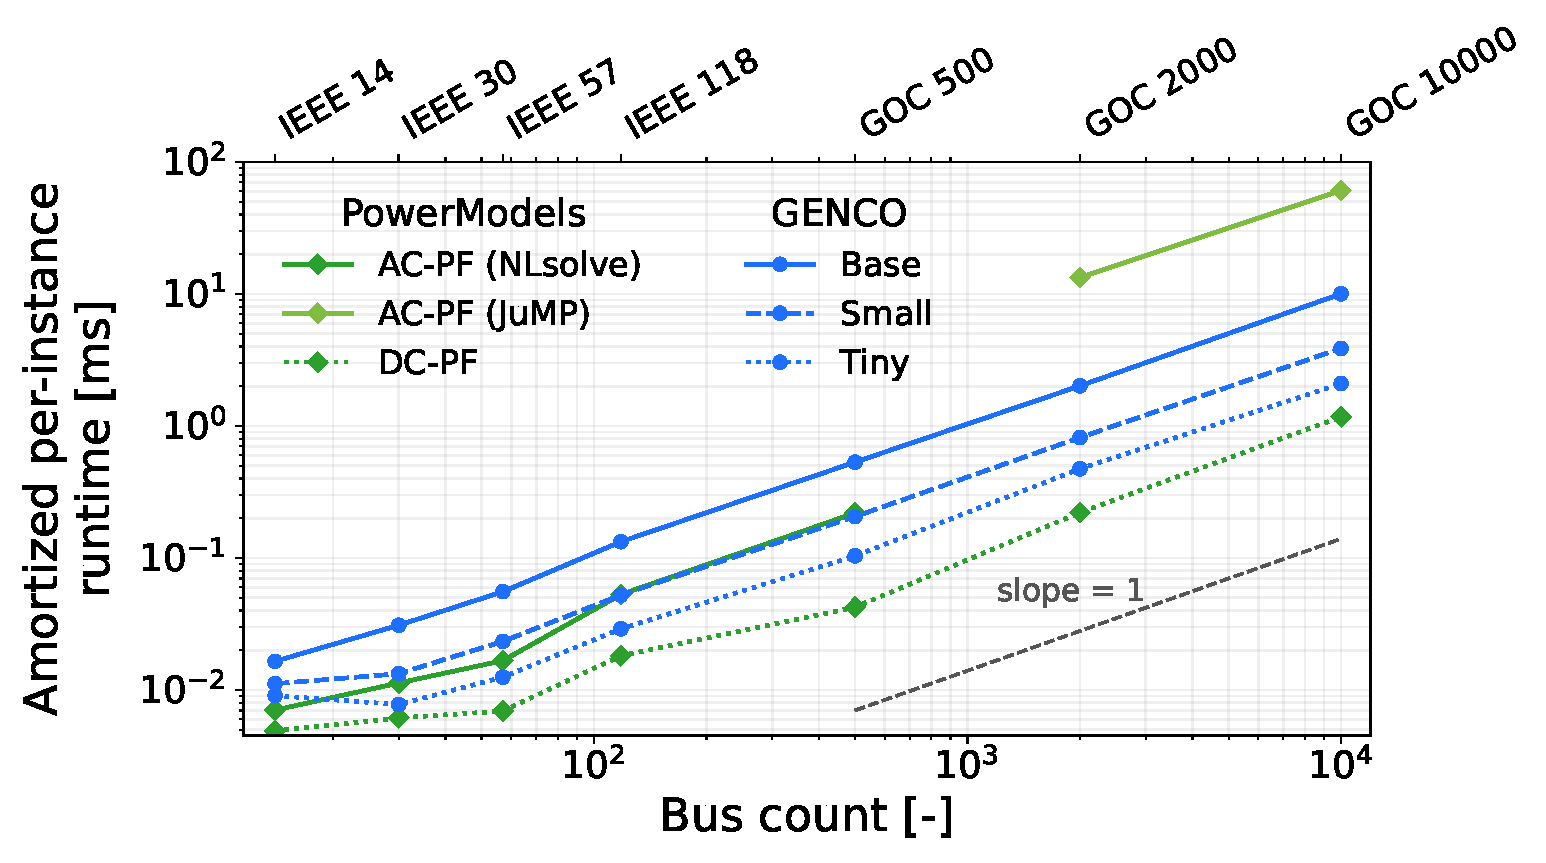
\includegraphics[width=\linewidth]{figures/runtime_analysis/runtime_comparison_from_raw_pf.pdf}
    \caption{Amortized per-instance runtime versus grid size for \genco and PowerModels AC-PF and DC-PF at the best batch size or worker count. Scaling exponents fitted on the four largest grids (two for AC-PF) are comparable across all methods, ranging from 0.94 to 0.97.}
    \label{fig:gridsize_runtime_pf}
\end{figure}


\begin{figure}
    \centering
    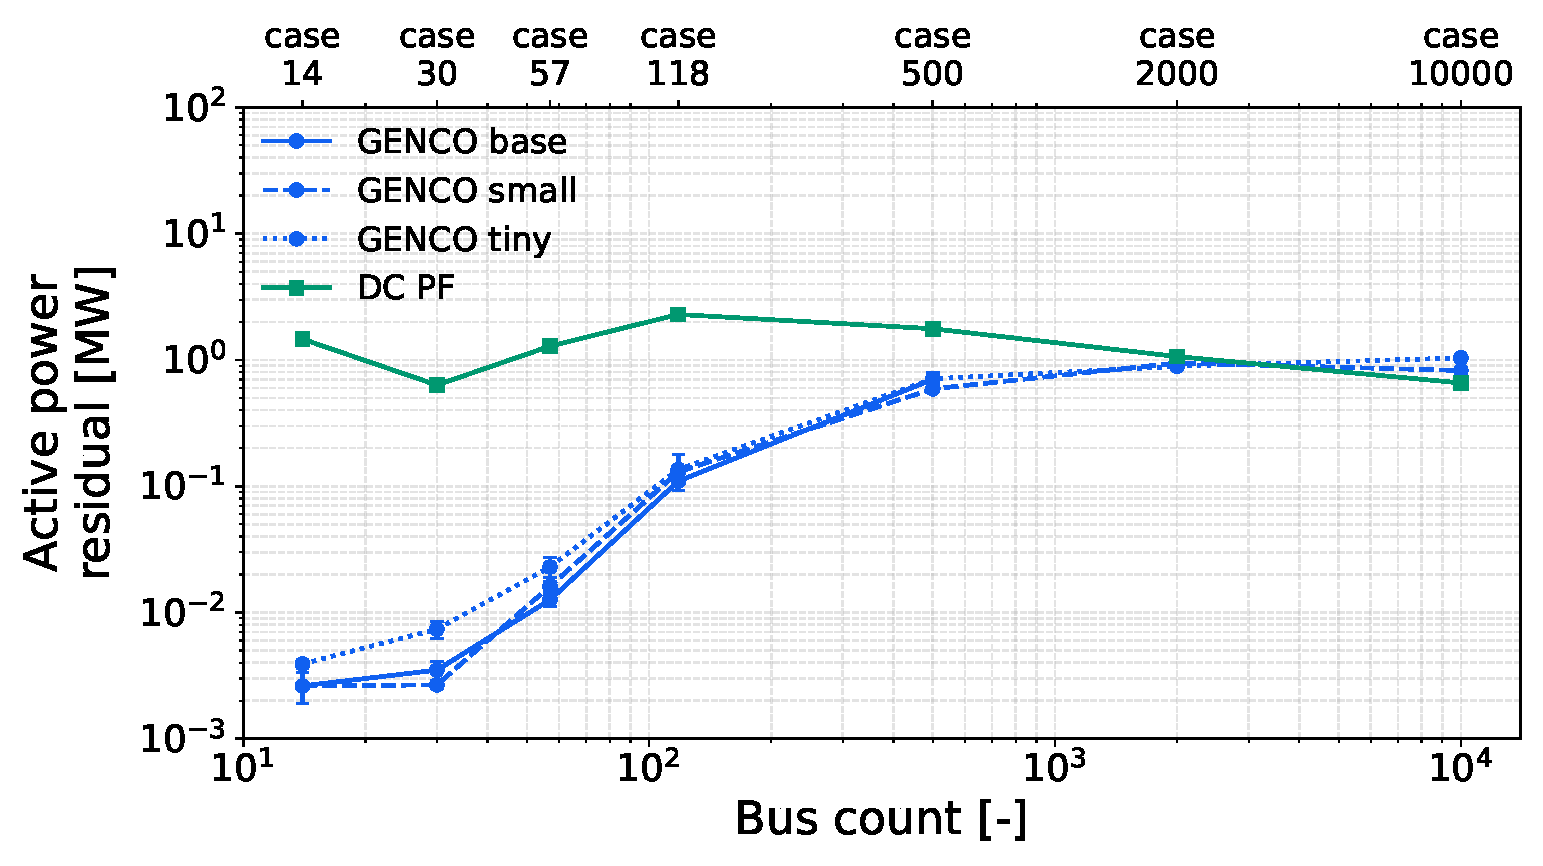
\includegraphics[width=1\linewidth]{figures/runtime_analysis/grid_scaling_active_residuals_pf.pdf}
    \caption{Mean active power-balance residuals versus grid size for \genco and PowerModels DC-PF.}
   \label{fig:gridsize_vs_residuals_pf}
\end{figure}


\paragraph{Runtime and accuracy for different grid sizes.}
The amortized per-instance runtime of \genco, AC-PF, and DC-PF as a function of bus count at the optimal batch size (\genco) or worker count (for the PowerModels-based classical solvers) is depicted in \cref{fig:gridsize_runtime_pf}. The runtime of all \genco versions (Base, Small, and Tiny) scales close to linear with grid size. For AC-PF, we selected the fastest converging solver available in PowerModels: the NLsolve-based solver for grids up to 500 buses and the JuMP-based solver for larger grids, as indicated by the disconnected lines. For large grids, the slopes of all solvers are similar, while for small networks AC-PF and DC-PF runtimes are nearly constant as multiprocessing overhead dominates. Active power-balance residuals are shown in \cref{fig:gridsize_vs_residuals_pf}. PowerModels AC-PF residuals ($10^{-11}$--$10^{-8}$~MW) are omitted for readability, while DC-PF remains near 1~MW. \genco increases from about $10^{-3}$~MW on the smallest IEEE grids to about 1~MW on GOC~2,000 and GOC~10,000. Its residuals are substantially lower than for DC-PF through GOC~500, slightly lower on GOC~2,000, and comparable to or slightly above for GOC~10,000, where Small outperforms Tiny; Base is evaluated only through GOC~500.\\





\paragraph{\genco's utility for PF.} \cref{tab:pf_selected_genco_tradeoff} summarizes the PF speed--accuracy trade-off, focusing on \genco Tiny because it provides the highest throughput while retaining useful solution accuracy: For a learned PF surrogate to be compelling, it must first provide a meaningful speedup over AC-PF, whose solutions are more accurate; modest gains may not offset the cost of training, maintaining, and deploying the neural solver. This criterion is not met on the small grids up to 500 buses, and the approximately $2\times$ speedup on GOC~500 remains marginal. In contrast, \genco Tiny is approximately $28$--$29\times$ faster than AC-PF on GOC~2,000 and GOC~10,000, making the learned approach increasingly attractive at scale. On these grids, \genco provides a good alternative to DC-PF: unlike DC-PF, it predicts a complete AC state, including voltage magnitudes and reactive generation, and therefore supports downstream voltage- and reactive-power-based analyses. For this reason, \genco can remain useful even when it is moderately slower or has slightly larger active power-balance residuals than DC-PF. On GOC~2,000 and GOC~10,000, it achieves similar residuals while being approximately $2\times$ slower than DC-PF. Overall, \genco Tiny is compelling for large-scale PF, where it substantially outperforms AC-PF and provides a complete AC state at a modest slowdown relative to DC-PF; on grids through GOC~500, AC-PF remains preferable.

\begin{table}
\centering
\scriptsize
\setlength{\tabcolsep}{3pt}
\renewcommand{\arraystretch}{1.1}
\begin{tabular}{@{}l c c c >{\raggedright\arraybackslash}p{0.35\linewidth}@{}}
\toprule
Grid
& \shortstack{Speedup\\vs AC-PF}
& \shortstack{DC-PF/\genco\\residual}
& \shortstack{Speedup\\vs DC-PF}
& Utility \\
\midrule
  14 & $0.8\times$ & $374.0\times$ & $0.5\times$ & 
  \multirow{5}{=}{None. Slower than AC-PF, which should be preferred since it provides more accurate solutions.} \\
  30 & $1.5\times$ & $85.8\times$ & $0.8\times$ &  \\
  57 & $1.3\times$ & $56.1\times$ & $0.6\times$ &  \\
 118 & $1.8\times$ & $16.9\times$ & $0.6\times$ &  \\
 500 & $2.1\times$ & $2.49\times$ & $0.4\times$ &  \\
\midrule
2000 & $28.2\times$ & $1.19\times$ & $0.5\times$ &
\multirow{6}{=}{\raggedright
Much faster than AC-PF; provides complete solutions with near-DC-PF active power-balance residuals at only 2× the runtime of DC-PF.} \\
10000 & $29.1\times$ & $0.63\times$ & $0.6\times$ & \\
& & & & \\
& & & & \\
& & & & \\
& & & & \\
\bottomrule
\end{tabular}
\caption{Scaling performance summary for \genco on Power Flow. Speedups $>$1 mean faster; the Utility column summarizes the recommended use of \genco relative to AC-PF and DC-PF for each grid-size. Results are for \genco Tiny for all grid sizes as it provides the best speedups and reasonable performance.}
\label{tab:pf_selected_genco_tradeoff}
\end{table}

\subsubsection{OPF Scaling with Grid Size: Runtime and Accuracy}

The amortized per-instance runtime as a function of grid size for AC-OPF, DC-OPF, and \genco is shown in \cref{fig:gridsize_runtime_opf}. The runtime values for \genco are independent of the task and thus identical to \cref{fig:gridsize_runtime_pf}. However, OPF is substantially harder to solve for classical solvers, resulting in a runtime advantage for \genco across all grid sizes.\\

% For a sequential comparison with CANOS, which reports per-sample solve times without parallelization, we use the best mean per-worker runtime from setup s2, which includes scenario parsing and solving.%
% % s2 best mean_pf_runtime_s worker counts: AC-OPF p=24 (GOC 500), p=24 (GOC 2000), p=40 (GOC 10000); DC-OPF p=24 (GOC 500), p=24 (GOC 2000), p=24 (GOC 10000).
% For AC-OPF, this yields 1.04~s for GOC~500, 6.65~s for GOC~2,000, and 51.5~s for GOC~10,000, compared to 6.49~s, 83.78~s, and 869.54~s, respectively, reported for AC-IPOPT before power-flow post-processing in CANOS~\cite{piloto2024}. These runtimes are approximately $6\times$ to $17\times$ lower. Our corresponding DC-OPF times (0.097~s, 0.457~s, and 3.19~s) are likewise about $9\times$ to $16\times$ lower than the CANOS DC-IPOPT before-power-flow runtimes (1.3~s, 4.27~s, and 50~s).




\begin{figure}
    \centering
    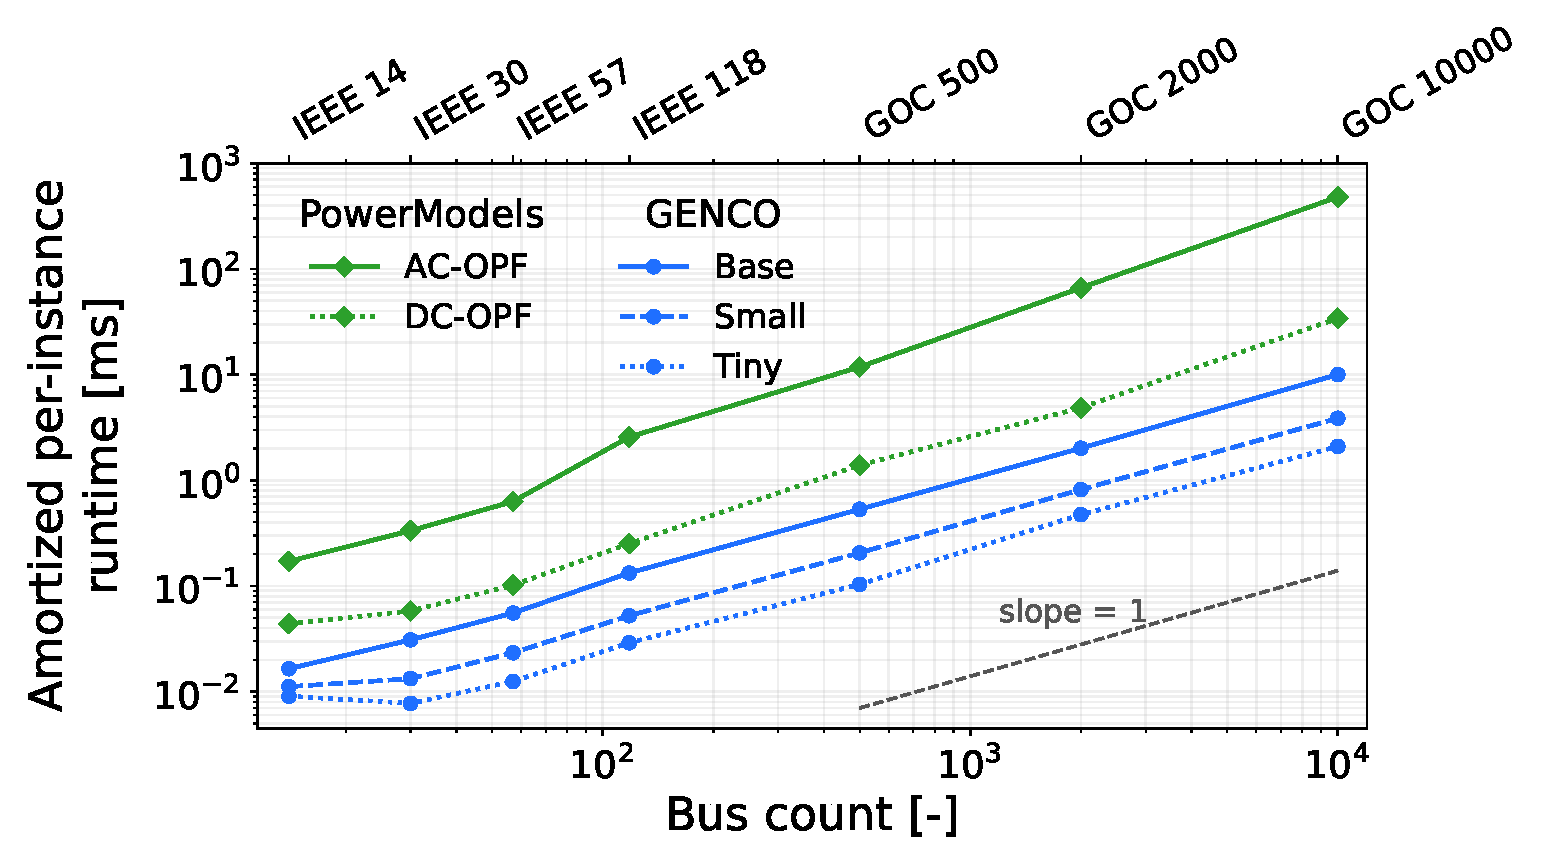
\includegraphics[width=\linewidth]{figures/runtime_analysis/runtime_comparison_from_raw_opf.pdf}
    \caption{Amortized per-instance runtime versus grid size for \genco and PowerModels AC-OPF and DC-OPF solvers. Results are reported for the optimal batch size for \genco and the best worker count for PowerModels. Four-largest-grid scaling exponents are 1.18 for AC-OPF, 1.09 for DC-OPF, and 0.97/0.95/0.94 for \genco Base/Small/Tiny.}
    \label{fig:gridsize_runtime_opf}
\end{figure}



\paragraph{\genco's utility for OPF.} The performance of \genco Small (which offers the best tradeoff between runtime, optimality, and feasibility) across grid sizes is summarized in \cref{tab:opf_selected_genco_tradeoff}. \genco is substantially faster than AC-OPF and DC-OPF on every grid, reaching an $84.5\times$ speedup over AC-OPF on GOC~2,000. It also produces more feasible and cost-effective solutions than DC-OPF, although these gains generally decrease with grid size. Finally, \genco predicts quantities unavailable from DC-OPF, including voltage magnitudes and reactive power setpoints. Overall, \genco offers a compelling alternative to DC-OPF. Detailed optimality and constraint-violation results for \genco Base and Small are reported in \cref{tab:opf_scaling} in the Appendix.\\



\begin{table}
\centering
\scriptsize
\setlength{\tabcolsep}{4pt}
\renewcommand{\arraystretch}{1.2}
% Requires \usepackage{booktabs}.
\begin{tabular}{@{}l c c c c@{}}
\toprule
Grid
& \shortstack{Speedup\\vs AC-OPF}
& \shortstack{Opt. gap reduction\\vs DC-OPF}
& \shortstack{Violation reduction\\vs DC-OPF}
& \shortstack{Speedup\\vs DC-OPF} \\
\midrule
  14 & $16.1\times$ & $55.2\times$ & $86.0\times$ & $4.14\times$ \\
  30 & $22.9\times$ & $31.8\times$ & $72.4\times$ & $3.99\times$ \\
  57 & $26.5\times$ & $6.28\times$ & $4.67\times$ & $4.29\times$ \\
 118 & $48.4\times$ & $2.85\times$ & $2.40\times$ & $4.75\times$ \\
 500 & $54.3\times$ & $3.20\times$ & $10.3\times$ & $6.40\times$ \\
2000 & $84.5\times$ & $1.85\times$ & $6.70\times$ & $6.19\times$ \\
\bottomrule
\end{tabular}
\caption{Performance scaling summary for \genco Small on Optimal Power Flow; Speedups $>$1 mean faster; optimality and feasibility improvements are ratios of DC-OPF to \genco mean metrics.}
\label{tab:opf_selected_genco_tradeoff}
\end{table}



\begin{boxH}
\paragraph{Takeaways.}

\begin{itemize}

% \item We introduced a method to perform a fair run-time assessment with i) fully utilized CPU and GPU, ii) the choice of sufficiently large benchmark scenarios, iii) the definition of the wall-clock time, and iv) the selection of equivalent compute hardware. 

\item For PF, \genco starts providing a valuable alternative to DC-PF for large grids ($\geq$2000 buses) by predicting the full AC operating state, including voltage magnitudes and reactive power, while achieving active power-balance residuals comparable to DC-PF, with up to \maxpfspeedups speedup over Newton--Raphson and only a \dcpfspeedupovergenco runtime relative to DC-PF.

\item For OPF, \genco is compelling across all evaluated grid sizes: Small is $16$--$85\times$ faster than AC-OPF and $4$--$6\times$ faster than DC-OPF, while reducing DC-OPF optimality gaps by $1.9$--$55\times$ and feasibility violations by $2.4$--$86\times$.



\end{itemize}
\end{boxH}